\documentclass[presentation,aspectratio=43]{beamer}

\usepackage{tikz}
\usetikzlibrary{positioning,calc}
\usetikzlibrary{shapes.geometric}
\usetikzlibrary{backgrounds}% only to show the bounding box
\usetikzlibrary{shapes,arrows}
\usepackage{appendixnumberbeamer}
\usepackage{amsmath}
\usepackage{ifxetex}
\ifxetex
\else
\usepackage[utf8]{inputenc}
\fi
\newif\ifwidescreen
\widescreenfalse
\date{12th June 2017}
\usetheme{firedrake}

\renewcommand{\vec}[1]{\ensuremath{\boldsymbol{#1}}}
\newcommand{\ddt}[1]{\frac{\partial #1}{\partial t}}
\newcommand{\zhat}{\hat{\vec{z}}}
\newcommand{\W}{\ensuremath{\mathbb{W}}}

\newcommand{\inner}[1]{\left\langle #1 \right \rangle}

\newcommand{\KSP}[2]{\ensuremath{\mathcal{K}\left(#1, \mathbb{#2}\right)}}
\newcommand{\ksp}[1]{\KSP{#1}{#1}}

\newcommand{\colourfiredrake}[1]{\colorbox{red!20}{#1}}
\newcommand{\colourpetsc}[1]{\colorbox{blue!20}{#1}}

\author{Lawrence Mitchell\inst{1,*} \and Rob Kirby\inst{2}}
\institute{
\inst{1}Departments of Computing and Mathematics, Imperial College
London

\inst{*}\texttt{lawrence.mitchell@imperial.ac.uk}
\and
\inst{2}Department of Mathematics, Baylor University
}

\graphicspath{{./\jobname.figures/}}
\newenvironment{changemargin}[2]{%
  \begin{list}{}{%
    \setlength{\topsep}{0pt}%
    \setlength{\leftmargin}{#1}%
    \setlength{\rightmargin}{#2}%
    \setlength{\listparindent}{\parindent}%
    \setlength{\itemindent}{\parindent}%
    \setlength{\parsep}{\parskip}%
  }%
  \item[]}{\end{list}}

\usepackage[url=false,
            doi=true,
            isbn=false,
            style=authoryear,
            firstinits=true,
            uniquename=init,
            backend=biber]{biblatex}

\setbeamertemplate{bibliography item}{}
\renewcommand{\bibfont}{\fontsize{7}{7}\selectfont}
\addbibresource{references.bib}
\newcommand{\arxivlink}[2]{%
  \href{http://www.arxiv.org/abs/#1}%
  {{\small\texttt{arXiv:\,#1\,[#2]}}}%
}

\setlength{\bibitemsep}{1ex}
\setlength{\fboxsep}{1pt}

\renewbibmacro{in:}{}
\DeclareFieldFormat[article]{volume}{\textbf{#1}}
\DeclareFieldFormat{doi}{%
  doi\addcolon%
  {\ifhyperref{\href{http://dx.doi.org/#1}{\nolinkurl{#1}}}
    {\nolinkurl{#1}}}}
\AtEveryBibitem{%
\clearfield{pages}%
\clearfield{issue}%
\clearfield{number}%
}

\usepackage{minted}

\title{Across the great divide}
\subtitle{composable block preconditioning from UFL}
\begin{document}

\maketitle

\begin{frame}[fragile,t]
  \frametitle{UFL makes it easy to write complex PDEs}
  \begin{columns}
    \begin{column}{0.47\framewidth}
      \small
      \begin{block}{Rayleigh-B\'enard convection}
        \begin{equation*}
          \begin{split}
            -\Delta u + u\cdot\nabla u + \nabla p +
            \frac{\text{Ra}}{\text{Pr}} \hat{g}T &= 0 \\
            \nabla \cdot u &= 0 \\
            - \frac{1}{\text{Pr}} \Delta T + u\cdot \nabla T &= 0
          \end{split}
        \end{equation*}
      \end{block}
    \end{column}
    \begin{column}{0.52\framewidth}
\begin{minted}[fontsize=\tiny]{python}
from firedrake import *
mesh = Mesh(...)
V = VectorFunctionSpace(mesh, "CG", 2)
W = FunctionSpace(mesh, "CG", 1)
Q = FunctionSpace(mesh, "CG", 1)
Z = V * W * Q
Ra = Constant(200)
Pr = Constant(6.18)
upT = Function(Z)
u, p, T = split(upT)
v, q, S = TestFunctions(Z)
bcs = [...] # no-flow + temp gradient
nullspace = MixedVectorSpaceBasis(
   Z, [Z.sub(0), VectorSpaceBasis(constant=True),
       Z.sub(2)])
F = (inner(grad(u), grad(v))
     + inner(dot(grad(u), u), v)
     - inner(p, div(v))
     + (Ra/Pr)*inner(T*g, v)
     + inner(div(u), q)
     + inner(dot(grad(T), u), S)
     + (1/Pr) * inner(grad(T), grad(S)))*dx

solve(F == 0, upT, bcs=bcs, nullspace=nullspace)
\end{minted}
    \end{column}
  \end{columns}
\end{frame}


\begin{frame}[fragile]
  \begin{columns}
    \begin{column}{0.5\textwidth}
      \begin{block}{Cahn-Hilliard}
        \small
        \begin{align*}
          \phi_t - \nabla \cdot M \nabla \mu &= 0\\
          \mu - \frac{\text{d} f}{\text{d} \phi} + \lambda \Delta \phi &= 0\\
        \end{align*}
        Implicit timestepping
        \begin{equation*}
          \begin{bmatrix}
            \frac{\phi_{n+1} - \phi_n}{\Delta t} - \nabla \cdot M \nabla \mu_{n+\theta}\\
            \mu_{n+1} - \frac{\text{d} f_{n+1}}{\text{d} \phi_{n+1}} -
            \lambda \nabla^2\phi_{n+1}
          \end{bmatrix} = 0
        \end{equation*}
      \end{block}
    \end{column}
    \begin{column}{0.5\textwidth}
\begin{minted}[fontsize=\tiny,escapeinside=||]{python}
from firedrake import *
mesh = Mesh(...)
V = FunctionSpace(mesh, "CG", 1)
Z = V*V
|$\theta$| = 0.5
|$\lambda$| = Constant(0.005)
M = Constant(10)
q, v = TestFunctions(Z)
z = Function(Z)
z0 = Function(Z)
|$\phi_{n+1}$|, |$\mu_{n+1}$| = split(z)
|$\phi_n$|, |$\mu_n$| = split(z0)
|$\phi_{n+1}$| = variable(|$\phi_{n+1}$|)
f = 10*(|$\phi_{n+1}$|**2 - 1)**2
dfdphi = diff(f, |$\phi_{n+1}$|)
|$\mu_{n+\theta}$| = (1-|$\theta$|)*|$\mu_n$| + |$\theta$|*|$\mu_{n+1}$|
dt = 5e-6
F = ((|$\phi_{n+1}$| - |$\phi_n$|)*q
     + dt*M*dot(grad(|$\mu_{n+\theta}$|), grad(q))
     + (|$\mu_{n+1}$| - dfdphi)*v
     -|$\lambda$|*dot(grad(|$\phi_{n+1}$|), grad(v)))*dx
while t < ...:
    z0.assign(z)
    solve(F == 0, z)
\end{minted}
    \end{column}
  \end{columns}
\end{frame}

\begin{frame}[fragile]
  \begin{columns}
    \begin{column}{0.5\textwidth}
      \begin{block}{Ohta-Kawasaki}
        \small
        \begin{align*}
          u_t - \Delta w + \sigma(u - m) &= 0\\
          w + \epsilon^2 \Delta u - u(u^2 - 1) &= 0
        \end{align*}
        Implicit timestepping + Newton
        \begin{equation*}
          \begin{bmatrix}
            (1 + \Delta t \theta \sigma)M  & \Delta t\theta K \\
            -\epsilon^2 K - M_E & M
          \end{bmatrix}
          \begin{bmatrix}
            \delta u \\
            \delta w
          \end{bmatrix} =
          \begin{bmatrix}
            f_1 \\
            f_2
          \end{bmatrix}
        \end{equation*}
      \end{block}
    \end{column}
    \begin{column}{0.5\textwidth}
\begin{minted}[fontsize=\tiny,escapeinside=||]{python}
from firedrake import *
mesh = Mesh(...)
V = FunctionSpace(mesh, "CG", 1)
Z = V*V
|$\epsilon$| = Constant(0.02)
|$\sigma$| = Constant(100)
dt = Constant(eps**2)
|$\theta$| = Constant(0.5)
v, q = TestFunctions(Z)
z = Function(Z)
z0 = Function(Z)
u, w = split(z)
u0, w0 = split(z0)
u|$_\theta$| = (1 - |$\theta$|)*u0 + |$\theta$|*u
w|$_\theta$| = (1 - |$\theta$|)*w0 + |$\theta$|*w
dfdu = u**3 - u
F = ((u - u0)*v
     + dt*dot(grad(w|$_\theta$|), grad(v))
     + dt*|$\sigma$|*(u|$_\theta$| - m)*v
     + w*q - dfdu*q
     - |$\epsilon$|**2*dot(grad(u), grad(q)))*dx
while t < ...:
    z0.assign(z)
    solve(F == 0, z)
\end{minted}
    \end{column}
  \end{columns}
\end{frame}

\begin{frame}[t]
  \frametitle{What about the solvers?}
  \begin{itemize}
  \item LU is alright for small problems
  \item \dots but quickly becomes untenable in 3D.
  \item Instead we use iterative methods (e.g.~Krylov methods)
  \item<2-> \dots but Krylov methods are \emph{not} solvers
  \item<3-> so we need \emph{preconditioners}.
  \end{itemize}
\end{frame}
\begin{frame}
  \frametitle{Block preconditioning}
  \begin{itemize}
  \item Coupled problems are (typically) not amenable to black
    box preconditioning.
  \item<2-> Solution: block preconditioning
  \end{itemize}
  \begin{columns}<2>[t]
    \begin{column}{0.5\textwidth}
      \begin{block}{Schur complement}
        \begin{equation*}
          T = \begin{bmatrix}
            A & 0 \\
            0 & C A^{-1} B^T
          \end{bmatrix}^{-1}
          \begin{bmatrix}
            A & B^T \\
            C & 0
          \end{bmatrix}
        \end{equation*}
        has minimal polynomial $T(T - I)(T^2 - T - I) = 0$.
        \nocite{Murphy:2000,Ipsen:2001,Benzi:2005}
      \end{block}
    \end{column}
    \begin{column}{0.5\textwidth}
      \begin{block}{Function space}
        If $\mathcal{A} : W \rightarrow W^*$, then
        \begin{equation*}
          \langle u, v \rangle_W^{-1} \mathcal{A}
        \end{equation*}
        has mesh independent condition number.
        \nocite{Malek:2014,Mardal:2011,Kirby:2010}
      \end{block}
    \end{column}
  \end{columns}
\end{frame}

\begin{frame}
  \frametitle{A problem}
  \begin{itemize}
  \item Such preconditioners often need auxiliary matrices not
    appearing the original operator.
  \item How do we provide these to the solver library in a composable
    manner?
  \end{itemize}
  \begin{block}<2->{Firedrake \& PETSc to the rescue}
  \begin{itemize}
  \item PETSc already provides a highly runtime-configurable library
    for \emph{algebraically} composing solvers. \nocite{Brown:2012}

  \item Firedrake makes it straightforward to build auxiliary
    operators.

  \item We combine these to allow simple development of complex
    preconditioners.
  \end{itemize}
  \end{block}
\end{frame}
\begin{frame}[fragile,t]
  \frametitle{Two new pieces}
  \begin{block}{A new matrix type}
    A PETSc shell matrix that implements matrix-free actions using
    Firedrake, and contains the UFL of the bilinear form.
    \begin{columns}
      \begin{column}{0.5\textwidth}
      \begin{equation*}
        y \leftarrow A x
      \end{equation*}
    \end{column}
    \hspace{-0.1\textwidth}
    \begin{column}{0.7\textwidth}
\begin{minted}[fontsize=\scriptsize]{python}
A = assemble(a, mat_type="matfree")
\end{minted}
    \end{column}
    \end{columns}
  \end{block}
  \vspace{1.5\baselineskip}
  \begin{block}{Custom preconditioners}
    Such matrices do not have entries, we create preconditioners
    that inspect the UFL and do the appropriate thing.
    \begin{columns}
      \begin{column}{0.5\textwidth}
    \begin{equation*}
      y \leftarrow \tilde{A}^{-1} x
    \end{equation*}
  \end{column}
  \hspace{-0.1\textwidth}
  \begin{column}{0.7\textwidth}
\begin{minted}[fontsize=\scriptsize]{python}
solve(a == L, x,
      {"pc_type": "python",
       "pc_python_type": "AssembledPC"})
\end{minted}
  \end{column}
  \end{columns}
  \end{block}
\end{frame}
\begin{frame}[fragile,t]
  \frametitle{A simple example}
  Matrix-free actions with AMG on the assembled operator.
  \vspace{2\baselineskip}
  \begin{columns}
    \begin{column}[b]{0.5\textwidth}
\begin{minted}[fontsize=\tiny,escapeinside=||]{python}
a = u*v*dx + dot(grad(u), grad(v)*dx)
opts = {|\colourpetsc{”ksp\_type”: ”cg”}|,
        |\colourfiredrake{”mat\_type”: ”matfree”}|,
        |\colourfiredrake{”pc\_type”: ”python”}|,
        |\colourfiredrake{”pc\_python\_type”: ”AssembledPC”}|,
        |\colourpetsc{”assembled\_pc\_type”: ”hypre”}|}
solve(a == L, x, solver_parameters=opts)
\end{minted}
    \end{column}
    \ifwidescreen
    \begin{column}{0.5\textwidth}
    \else
    \hspace{-0.1\textwidth}
    \begin{column}{0.6\textwidth}
    \fi
      \begin{tikzpicture}[scale=0.7, every node/.style={transform shape},
        firedrake/.style={rounded rectangle,draw,black, fill=red!20, minimum size=6mm, inner sep=2pt},
        petsc/.style={rectangle,draw,black, minimum size=6mm,
          fill=blue!20, inner sep=2pt},
        arrow/.style={-stealth,line width=1}]
        \node[petsc] (ainv)
        {$A^{-1} \approx \mathcal{K}(A, A_p^{-1})$};
        \node[firedrake, below left=of ainv] (Ax) {$Ax$};
        \node[firedrake,below=of Ax] (ax)
        {\texttt{assemble(action(a, x))}};
        \node[petsc,below right=of ainv] (ap) {$A_p^{-1}$};
        \node[firedrake,below=of ap] (Ap)
        {$A_p
          \leftarrow$\raisebox{0.75pt}{\texttt{assemble(a)}}};
        \node[petsc,below=of Ap] (Apinv)
        {\texttt{hypre($A_p$)}};

        \draw[arrow] (ainv) -- (Ax); \draw[arrow] (Ax) -- (ax);
        \draw[arrow] (ainv) -- (ap); \draw[arrow] (ap) -- (Ap);
        \draw[arrow] (Ap) -- (Apinv);
      \end{tikzpicture}
    \end{column}
  \end{columns}
\end{frame}
\bgroup
\setbeamertemplate{background}{}
\begin{frame}[plain]
  \begin{tikzpicture}[remember picture,overlay]
    \node[at=(current page.center)] {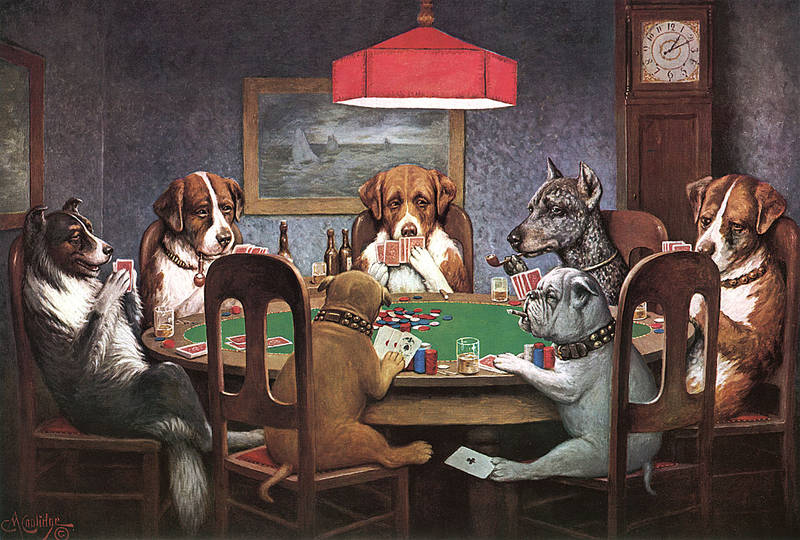
\includegraphics[width=\paperwidth]{underhand}};
  \end{tikzpicture}
\end{frame}
\egroup

\begin{frame}[allowframebreaks]
  \frametitle{Something more complicated}
  A preconditioner for the Ohta--Kawasaki equation
  \parencite{Farrell:2016}
  \begin{equation*}
    \begin{split}
      u_t - \Delta w + \sigma(u - m) &= 0\\
      w + \epsilon^2 \Delta u - u(u^2 - 1) &= 0
    \end{split}
  \end{equation*}
  Newton iteration at each timestep solves
  \begin{equation*}
    \begin{bmatrix}
      (1 + \Delta t \theta \sigma)M  & \Delta t\theta K \\
      -\epsilon^2 K - M_E & M
    \end{bmatrix}
    \begin{bmatrix}
      \delta u \\
      \delta w
    \end{bmatrix} =
    \begin{bmatrix}
      f_1 \\
      f_2
    \end{bmatrix}
  \end{equation*}
  \pagebreak

  Preconditioning strategy:
  {\scriptsize
    \begin{equation*}
      \begin{bmatrix}
        \left[(1 + \Delta t \theta \sigma)M\right]^{-1}  & 0 \\
        0 & S^{-1}
      \end{bmatrix}
      \begin{bmatrix}
        I & 0\\
        (\epsilon^2 K + M_E)\left[(1 + \Delta t \theta
          \sigma)M\right]^{-1} & I\\
      \end{bmatrix}
      \begin{bmatrix}
        (1 + \Delta t \theta \sigma)M  & \Delta t\theta K \\
        -\epsilon^2 K - M_E & M
      \end{bmatrix}.
    \end{equation*}
  }
  Where
  \begin{equation*}
    S = M + (\epsilon^2 K + M_E) \left[(1 + \Delta t\theta\sigma)M\right]^{-1} \Delta t \theta K
  \end{equation*}
  is inverted iteratively, preconditioned by
  \begin{equation*}
    S^{-1} \approx S_p^{-1} = \hat{S}^{-1}M\hat{S}^{-1}
  \end{equation*}
  with
  \begin{equation*}
    \hat{S} = M + \epsilon\sqrt{(\Delta t \theta)/(1+\Delta t \theta\sigma)} K.
  \end{equation*}
\end{frame}

\begin{frame}[fragile]
  \frametitle{Implementation}
\begin{minted}[fontsize=\tiny,mathescape,escapeinside=||]{python}
class OKPC(PCBase):

    def initialize(self, pc):
        # Approximate $S^{-1} \sim \hat{S}^{-1} M \hat{S}^{-1}$ where $\hat{S} = \inner{q, w} + \epsilon\sqrt{c}\inner{\nabla q, \nabla w}$, $c = \frac{\Delta t \theta}{1 + \Delta t \theta \sigma}$
        _, P = pc.getOperators()
        ctx = P.getPythonContext()
        # User information about $\Delta t$, $\theta$, etc...
        dt, |$\theta$|, |$\epsilon$|, |$\sigma$| = ctx.appctx["parameters"]
        V = ctx.a.arguments()[0].function_space()
        c = (dt * |$\theta$|)/(1 + dt * |$\theta$| * |$\sigma$|)
        w = TrialFunction(V)
        q = TestFunction(V)
        op = assemble(inner(w, q)*dx + |$\epsilon$|*sqrt(c)*inner(grad(w), grad(q))*dx)
        self.ksp = KSP().create(comm=pc.comm)
        self.ksp.setOptionsPrefix(pc.getOptionsPrefix + "shat_")
        self.ksp.setOperators(op.petscmat, op.petscmat)
        self.ksp.setFromOptions()
        mass = assemble(w*q*dx)
        self.mass = mass.petscmat
        work = self.mass.createVecLeft()
        self.work = (work, work.duplicate())

    def apply(self, pc, x, y):
        tmp1, tmp2 = self.work
        self.ksp.solve(x, tmp1)
        self.mass.mult(tmp1, tmp2)
        self.ksp.solve(tmp2, y)
\end{minted}
\end{frame}

\bgroup
\setbeamertemplate{background}{}
\setbeamercolor{footline}{
  use=normal text,
  fg=normal text.fg
}

\begin{frame}[fragile]
  \frametitle{Usage}
  \begin{columns}
    \ifwidescreen
    \begin{column}{0.5\textwidth}
    \else
    \hspace{-0.8cm}
    \begin{column}{0.35\textwidth}
    \fi
\begin{minted}[fontsize=\tiny,escapeinside=||]{py}
opts = {
  "snes_lag_preconditioner": -1,
  |\colourfiredrake{”mat\_type”: ”matfree”}|,
  |\colourpetsc{”ksp\_type”: ”gmres”}|,
  |\colourpetsc{”pc\_type”: ”fieldsplit”}|,
  |\colourpetsc{”pc\_fieldsplit\_type”: ”schur”}|,
  |\colourpetsc{”pc\_fieldsplit\_schur\_factorization\_type”: ”lower”}|,
  |\colourpetsc{”fieldsplit\_0”}|: {
     |\colourpetsc{”ksp\_type”: ”chebyshev”}|,
     "ksp_max_it": 10,
     |\colourfiredrake{”pc\_type”: ”python”}|,
     |\colourfiredrake{”pc\_python\_type”: ”firedrake.AssembledPC”}|,
     |\colourpetsc{”assembled\_pc\_type”: ”sor”}|},
  |\colourpetsc{”fieldsplit\_1”}|: {
     |\colourpetsc{”ksp\_type”: ”richardson”}|,
     "ksp_max_it": 2,
     |\colourfiredrake{”pc\_type”: ”python”}|,
     |\colourfiredrake{”pc\_python\_type”: ”OKPC”}|,
     |\colourpetsc{”shat\_ksp\_type”: ”richardson”}|,
     "shat_ksp_max_it": 5,
     |\colourpetsc{”shat\_pc\_type”: ”hypre”}|
 }

appctx = {"parameters": (dt, theta, eps, sigma)}
solve(L == 0, z, solver_parameters=opts, appctx=appctx)
\end{minted}
  \end{column}
  \ifwidescreen
  \hspace{-0.05\textwidth}
  \begin{column}{0.55\textwidth}
  \else
  \begin{column}{0.65\textwidth}
  \fi
  \begin{tikzpicture}[scale=0.55, every node/.style={transform shape},
    firedrake/.style={rounded rectangle,draw,black, fill=red!20, minimum size=6mm, inner sep=2pt},
    petsc/.style={rectangle,draw,black, fill=blue!20, minimum size=6mm, inner sep=2pt},
    arrow/.style={-stealth,line width=0.8}]
    \node[petsc] (Jinv) {$J^{-1} \approx \mathcal{K}(J,
      J_p^{-1})$};
    \node[firedrake, below left=0.1cm and 0.3cm of ainv.south west] (Jx) {$Jx$};
    \node[firedrake,below=0.5cm of Jx.south] (jx) {\texttt{assemble(action(J, x))}};
    \node[petsc,below right=0.5cm and -0.1cm of Jinv] (Jpinv) {$J_p^{-1} =%
      \left[%
        \begin{smallmatrix}
          A^{-1} & 0\\
          0 & S^{-1}
        \end{smallmatrix}%
      \right]
      \left[%
      \begin{smallmatrix}
        I & 0 \\
        -CA^{-1} & 0 \\
      \end{smallmatrix}%
      \right]
      $};
    \node[petsc, below left=0.8cm and -1cm of Jpinv] (Ainv)  {$A^{-1}\approx \mathcal{K}(A,A_p^{-1})$};
    \node[firedrake, below left=1cm and 1.5cm of Ainv] (Ax) {$Ax$};
    \node[firedrake, below=3cm of Ax] (ax) {\texttt{assemble(action(A, x))}};
    \node[firedrake, below=1.5cm of Ainv] (Ap)
    {$A_p \leftarrow \text{\raisebox{0.5pt}{\texttt{assemble(A\_p)}}}$};
    \node[petsc, below=of Ap] (Apinv) {\texttt{SOR($A_p$)}};

    \node[petsc, below=1.3cm of Jpinv.south east, anchor=north] (Sinv) {$S^{-1} \approx \mathcal{K}(S,
      S_p^{-1})$};
    \node[petsc, below left=2cm and 0.3cm of Sinv, anchor=north] (S) {$Sx = (M - C A^{-1} B)x$};
    \node[firedrake, below=of S] (Cx) {$Cx$};
    \node[firedrake, right=of Cx] (Mx) {$Mx$};
    \node[firedrake, left=of Cx] (Bx) {$Bx$};

    \node[firedrake, below=1.5cm of Cx] (actionx) {\texttt{assemble(action($\cdot$, x))}};

    \node[firedrake, below right=0.8cm and -0.2cm of Sinv, anchor=north] (Spinv) {$S_p^{-1} = \hat{S}^{-1} M
      \hat{S}^{-1}$};
    \node[petsc, below=3.25cm of Spinv] (Shatinv) {$\hat{S}^{-1}
      \approx \mathcal{K}(\hat{S}, \hat{S}_p^{-1})$};
    \node[firedrake, below=1.5cm of Shatinv] (Shat)
    {$\hat{S}\text{\raisebox{0.5pt}{ $\leftarrow$ \texttt{assemble(s\_hat)}}}$};
    \node[petsc, below=1cm of Shat] (Shathypre) {\texttt{hypre($\hat{S}$)}};

    \draw[arrow] (Jinv.south west) -- (Jx);
    \draw[arrow] (Jx) -- (jx);
    \draw[arrow] (Jinv.south east) -- (Jpinv);

    \draw[arrow] (Jpinv.south west) -- (Ainv.north);
    \draw[arrow] (Ainv.south west) -- (Ax);
    \draw[arrow] (Ax) -- (ax);
    \draw[arrow] (Ainv) -- (Ap);
    \draw[arrow] (Ap) -- (Apinv);
    \draw[arrow] (Jpinv) -- (Sinv);
    \draw[arrow] (Sinv) -- (S);
    \draw[arrow] (S) -- (Ainv.south east);

    \draw[arrow] (S) -- (Bx);
    \draw[arrow] (S) -- (Cx);
    \draw[arrow] (S) -- (Mx);

    \draw[arrow] (Bx) -- (actionx);
    \draw[arrow] (Cx) -- (actionx);
    \draw[arrow] (Mx) -- (actionx);

    \draw[arrow] (Sinv) -- (Spinv);
    \draw[arrow] (Spinv) -- (Mx);
    \draw[arrow] (Spinv) -- (Shatinv);
    \draw[arrow] (Shatinv) -- (Shat);
    \draw[arrow] (Shat) -- (Shathypre);
  \end{tikzpicture}
    \end{column}
  \end{columns}
\end{frame}
\begin{frame}
  \frametitle{Conclusions}

  \begin{itemize}
  \item Composable, extensible method using UFL to build block
    preconditioners.

  \item Model formulation doesn't need to know about the solver
    configuration.

  \item Composes with nonlinear solvers that need linearisations: no
    need to write your own special Newton iteration to get data in.

  \item Automatically takes advantage of any improvements in Firedrake
    (fast matrix actions, etc...)

  \end{itemize}

  \begin{center}
    \textcite{Kirby:2017} \arxivlink{1706.01346}{cs.MS}

    \url{www.firedrakeproject.org}
  \end{center}
  \begin{tikzpicture}[remember picture,overlay]
    \node[at=(current page.south east), anchor=south east] {
\includegraphics[width=2.5cm]{epsrc-logo}};
  \end{tikzpicture}

\end{frame}


\appendix
\begin{frame}
  \frametitle{References}
  \printbibliography[heading=none]
\end{frame}
\egroup

\end{document}
